%% LyX 2.1.4 created this file.  For more info, see http://www.lyx.org/.
%% Do not edit unless you really know what you are doing.
\documentclass[a4paper,oneside,brazil,11pt,a4paper,openright,titlepage,usenames,dvipsnames]{book}
\usepackage[utf8]{inputenc}
\usepackage[T1]{fontenc}
\usepackage{lmodern}
\setcounter{secnumdepth}{3}
\setcounter{tocdepth}{3}
\usepackage{array}
\usepackage{verbatim}
\usepackage{calc}
\usepackage{textcomp}
\usepackage{amssymb}
\usepackage{graphicx}
\usepackage{float}

\makeatletter

%%%%%%%%%%%%%%%%%%%%%%%%%%%%%% LyX specific LaTeX commands.
\pdfpageheight\paperheight
\pdfpagewidth\paperwidth

%% Because html converters don't know tabularnewline
\providecommand{\tabularnewline}{\\}

%%%%%%%%%%%%%%%%%%%%%%%%%%%%%% User specified LaTeX commands.
% Classe alternativa, apropriada para impressão frente-verso. Inclui páginas em branco
% de forma que capítulos sempre tenham início na página à direita:
% \documentclass[11pt,a4paper,openright,titlepage]{book}

% Pacotes
\usepackage[T1]{fontenc}
\usepackage[brazilian]{babel}
\usepackage{epsfig}
\usepackage{subfigure}
\usepackage{amsfonts}
\usepackage{amsmath}
\usepackage[thmmarks,amsmath]{ntheorem}%\usepackage{amsthm}
\usepackage{boxedminipage}
\usepackage{geometry}
\usepackage{theorem}
\usepackage{fancybox}
\usepackage{fancyhdr}
\usepackage{ifthen}
\usepackage{xurl}
\usepackage{afterpage}
\usepackage{color}
\usepackage{colortbl}
\usepackage{rotating}
\usepackage{makeidx}
\usepackage{indentfirst}
% Pacotes para adição de figuras do inkscape
\usepackage{graphicx}
\usepackage{import}

% Escolher um dos seguintes formatos:
\usepackage{ft2unb} % segue padrão de fontes do Latex

\makeindex

\makeatother

\usepackage{babel}
\begin{document}
\setcounter{secnumdepth}{3}
\setcounter{tocdepth}{2}
\pagestyle{empty}

\grau{Engenheiro de Controle e Automação}

\tipodemonografia{TRABALHO DE GRADUAÇÃO}

\begin{comment}
Título
\end{comment}


\titulolinhai{MONITORAMENTO DE OCUPAÇÃO DE AMBIENTES}

\titulolinhaii{USANDO RFID PASSIVO}

\titulolinhaiii{}

\titulolinhaiv{}

\begin{comment}
Autores. Basta retirar o texto totalmente caso não haja um determinado
autor.
\end{comment}


\autori{André Abreu Rodrigues de Almeida}

\autorii{}

\autoriii{}

\begin{comment}
Membros da banca. Basta retirar o texto totalmente caso não haja um determinado membro da banca.
\end{comment}


\membrodabancai{Prof. Adolfo Bauchspiess, ENE/UnB}

\membrodabancaifuncao{Orientador}

\membrodabancaii{Prof. Lélio Ribeiro Soares Júnior, ENE/UnB}

\membrodabancaiifuncao{Examinador interno}

\membrodabancaiii{Eng. Ney César de Melo Filho}

\membrodabancaiiifuncao{Examinador externo}

\membrodabancaiv{}

\membrodabancaivfuncao{}

\membrodabancav{}

\membrodabancavfuncao{}

\begin{comment}
Data de defesa: mês e ano
\end{comment}


\mes{Dezembro}
\ano{2019}

\begin{comment}
Comandos para criar a capa e a página de assinaturas
\end{comment}


\capaprincipal
\capaassinaturas

\begin{comment}
Ficha Catalográfica
\end{comment}


\noindent \textbf{FICHA CATALOGRÁFICA}

\noindent %
\fbox{\begin{minipage}[t]{1\columnwidth}%
ANDRÉ, ABREU RODRIGUES DE ALMEIDA

Monitoramento de ocupação de ambientes utilizando RFID passivo


\medskip{}

{[}Distrito Federal{]} 2019.

\medskip{}


viii, 121p., 297 mm (FT/UnB, Engenheiro, Controle e Automação, 2019).
Trabalho de Graduação \textendash{} Universidade de Brasília. Faculdade
de Tecnologia.

\medskip{}


1. RFID\tab 2.Monitoramento%\hfill{}

3. RSSI\tab 4.Efeito Doppler%\hfill{}

\medskip{}


I. Mecatrônica/FT/UnB\tab II. Título (Série)%\hfill{}

%
\end{minipage}}

\noindent \medskip{}


\noindent \textbf{REFERÊNCIA BIBLIOGRÁFICA}

ALMEIDA, ANDRÉ ABREU RODRIGUES DE, (2019). Monitoramento de ocupação de ambientes utilizando RFID passivo. Trabalho de Graduação em Engenharia de Controle e Automação, Publicação FT.TG-$n^{\circ}022$,
Faculdade de Tecnologia, Universidade de Brasília, Brasília, DF, 121p.

\noindent \bigskip{}


\noindent \textbf{CESSÃO DE DIREITOS}

\noindent AUTOR: André Abreu Rodrigues de Almeida

TÍTULO DO TRABALHO DE GRADUAÇÃO: Monitoramento de ocupação de ambientes utilizando RFID passivo.

\noindent \medskip{}


\noindent GRAU: Engenheiro\hfill{}ANO: 2019\hfill{}

\noindent \medskip{}


É concedida à Universidade de Brasília permissão para reproduzir cópias
deste Trabalho de Graduação e para emprestar ou vender tais cópias
somente para propósitos acadêmicos e científicos. O autor reserva
outros direitos de publicação e nenhuma parte desse Trabalho de Graduação
pode ser reproduzida sem autorização por escrito do autor.

\noindent \bigskip{}


\noindent \rule[0.5ex]{1\columnwidth}{1pt}

\noindent André Abreu Rodrigues de Almeida

\noindent UnB - Faculdade de Tecnologia, Campus Universitário Darcy Ribeiro, Brasília.

\noindent 70910-900 Brasília \textendash{} DF \textendash{} Brasil.


\begin{comment}
Dedicatória
\end{comment}


\frontmatter

\begin{comment}
Texto de dedicatória do primeiro autor.
\end{comment}


\dedicatoriaautori{um beijo pra minha mãe, pro meu pai, e pra você}

\begin{comment}
Texto de dedicatória do segundo autor. Caso não tenha um segundo autor,
este texto não será mostrado
\end{comment}


\dedicatoriaautorii{Dedicatória do autor 2}

\begin{comment}
Texto de dedicatória do terceiro autor. Caso não tenha um terceiro
autor, este texto não será mostrado
\end{comment}


\dedicatoriaautoriii{Dedicatória do autor 3}

\begin{comment}
Comando para criar a página de dedicatória
\end{comment}


\dedicatoria

\begin{comment}
Agradecimentos
\end{comment}


\begin{comment}
Texto de agradecimentos do primeiro autor.
\end{comment}


\agradecimentosautori{Agradecimentos!}

\begin{comment}
Texto de agradecimentos do segundo autor. Caso não tenha um segundo
autor, este texto não será mostrado.
\end{comment}


%\agradecimentosautorii{A inclusão desta seção de agradecimentos é opcional e fica à critério do(s) autor(es), que caso deseje(em) inclui-la deverá(ão) utilizar este espaço, seguindo esta formatação.}

\begin{comment}
Texto de agradecimentos do terceiro autor. Caso não tenha um terceiro
autor, este texto não será mostrado.
\end{comment}


%\agradecimentosautoriii{A inclusão desta seção de agradecimentos é opcional e fica à critério do(s) autor(es), que caso deseje(em) inclui-la deverá(ão) utilizar este espaço, seguindo esta formatação.}

\begin{comment}
Comando para criar a página de agradecimentos
\end{comment}


\agradecimentos

\resumo{resumo}{Resumo!

\medskip{}


Palavras Chave: bla, ble, bli

}\vspace*{2cm}


\resumo{Abstract}{Abstract, in English ofc!

\medskip{}


Keywords: bla, ble, bli

}

\begin{comment}
Listas de conteúdo, figuras e tabelas
\end{comment}


\sumario
\listadefiguras
\listadetabelas

\begin{comment}
Lista de Símbolos
\end{comment}


%TCIDATA{LaTeXparent=0,0,these.tex}


%\chapter*{\setfontarial\mdseries LISTA DE SÍMBOLOS} % se usar ft1unb.sty, descomente esta linha



\chapter*{LISTA DE SÍMBOLOS}

% se usar ft2unb.sty, descomente esta linha



\subsection*{Símbolos Latinos}

\begin{tabular}{p{0.1\textwidth}p{0.63\textwidth}>{\PreserveBacklash\raggedleft}p{0.15\textwidth}}
$v$  & Velocidade linear  & {[}m/s{]}\tabularnewline
\end{tabular}


\subsection*{Símbolos Gregos}

\begin{tabular}{p{0.1\textwidth}p{0.63\textwidth}>{\PreserveBacklash\raggedleft}p{0.15\textwidth}}
$\omega$ & Velocidade angular & {[}rad/s{]}\tabularnewline
\end{tabular}


\subsection*{Grupos Adimensionais}

\begin{tabular}{p{0.1\textwidth}p{0.8\textwidth}}
i, k & Contador\tabularnewline
\end{tabular}


\subsection*{Subscritos}

\begin{tabular}{p{0.1\textwidth}p{0.8\textwidth}}
$ref$  & referência \tabularnewline
$fer$  & ferramenta \tabularnewline
$sis$  & sistema \tabularnewline
$des$  & desejado\tabularnewline
\end{tabular}


\subsection*{Sobrescritos}

\begin{tabular}{p{0.1\textwidth}p{0.8\textwidth}}
$\cdot$  & Variação temporal \tabularnewline
$-$  & Valor médio \tabularnewline
\end{tabular}


\subsection*{Siglas}

\begin{tabular}{p{0.1\textwidth}p{0.8\textwidth}}
EPC  & Código Eletrônico do Produto - \textit{Electronic Product Code}\tabularnewline
GPS & Sistema de Posicionamento Global - \textit{Global Positioning System} \tabularnewline
HF & Alta Frequência - \textit{High Frequency} \tabularnewline
HVAC & Aquecimento, Ventilação e Ar-condicionado - \textit{Heating, Ventilation and Air Conditioning}\tabularnewline
IoT & Internet das coisas - \textit{Internet of Things} \tabularnewline
LARA & Laboratório de Automação e Robótica \tabularnewline
LF & Baixa Frequência - \textit{Low Frequency} \tabularnewline
RAIN & Identificação por radiofrequência - \textit{RAdio frequency IdentificatioN} \tabularnewline
RF & Radiofrequência - \textit{radiofrequency} \tabularnewline
RFID & Identificação por Radiofrequência - \textit{Radio Frequency Identification}\tabularnewline
UHF & Frequência Ultra Alta - \textit{Ultra High frequency} \tabularnewline
UnB & Universidade de Brasília \tabularnewline
\end{tabular}


\begin{comment}
Corpo Principal
\end{comment}


\mainmatter
\setcounter{page}{1}
\pagenumbering{arabic}
\pagestyle{plain}

\begin{comment}
Introdução
\end{comment}

\chapter{Introdução}

\label{CapIntro}

% Resumo opcional. Comentar se não usar.
\resumodocapitulo{O desenvolvimento tecnológico culminou na demanda por melhorias de serviços que, outrora, não eram capazes de integrar os fatores aliados à facilidade e ao bem-estar dos usuários. O bem-estar, dentro de edifícios, está associado diretamente ao conforto ambiental. Esse conceito é estudado nos ramos de arquitetura e construção civil e visa a garantia das condições que possibilitam a qualidade física e psicológica dos indivíduos dentro dos mais diversos ambientes e instalações.}

\section{Contextualização}

O momento em que se elabora este projeto é uma época de grandes mudanças em quesitos de tecnologia. O entendimento do impacto ao meio ambiente, gerado pelo consumo energético em residências, estabelecimentos comerciais e fabris começa a ser compreendido por boa parte das pessoas, e principalmente o conhecimento da escalabilidade do impacto individual das pessoas de uma população.

Nas últimas décadas, a racionalização do consumo energético vem sendo alvo de diversos encontros técnicos da área de sustentabilidade, e de diversos acordos globais para a redução das emissões de carbono, geradas principalmente, devido à ação humana, especialmente na produção de energia.

Ao mesmo tempo em que o consumo é questionado, as exigências quanto à qualidade de vida, segurança no trabalho, ergonomia e conforto passaram a ser aspectos chave na vida e no dia-a-dia das pessoas. Seja no trabalho, ou no ambiente domiciliar, o conforto térmico é decisivo para o bem-estar das pessoas, assim como para a produtividade no ambiente de trabalho.

É um desafio alcançar a completude do conceito de conforto ambiental nas edificações. Nesse sentido, a automação é capaz de otimizar situações de uso de instrumentos cotidianos para vantagens como: a facilitação de trabalhos, muitas vezes manuais, para a economia de energia, para o estabelecimento de relações automáticas entre duas variáveis, a exemplo da entrada de pessoas em uma sala e o acionamento do ar condicionado, dentre outras vantagens.

\subsection{Conforto ambiental}

Conforto Ambiental é um conjunto de condições que possibilitam o bem-estar físico e psicológico dos indivíduos em diferentes locais, sendo que, o enfoque deste trabalho é principalmente em relação ao interior de instalações.

Esse conforto pode ser subdividido em categorias como: visual (abrangendo iluminação e estética visual), ergonômico (que tem muito destaque na parte de segurança do trabalho e com exemplos claros de esforços repetitivos, etc.), acústico (onde há limites em decibéis muito bem definidos) e térmico, que se configura como objeto desse trabalho. As normas que regem a construção e habitação de ambientes quanto ao aspecto de conforto ambiental e térmico são as NBRs 15.575 \cite{NBR15575} e 15.220 \cite{NBR15220}.

\subsection{Tecnologias de comunicação sem fio}

O uso de RFID, Bluetooth, Zigbee pode auxiliar na automação e possibilitar a instalação de sistemas de condicionamento baseados na movimentação (entrada e saída) de pessoas. Segundo Ahmed et al. \cite{AhmedIntegrationStreamMapping}, sistemas wireless (sem fio) podem reduzir significativamente a frequência de erros humanos, otimizar a gestão e aumentar a acurácia da informação principalmente em relação à indoor network (rede interna). Chen et al. \cite{chenUsingRFID}, retrata ainda, quão importante é a utilização de ferramentas como o RFID para a rastreabilidade e compra segura de alimentos. O uso de RFID pode ser empregado até no controle do fluxo de saída de roupas de uma loja.

Esses sistemas que funcionam à distância, sem fio, como o RFID, que é o sistema de identificação por radiofreqüência (RFID), que será melhor explicado no capítulo \ref{chap:Fundamentacao}, permitem recuperar informações armazenadas de um objeto preso ou incorporado a bens, produtos ou seres vivos \cite{gutierrez2005complexo}. Dessa forma, o emprego de tecnologias sem fio pode proporcionar a melhor administração de indivíduos em situações rotineiras e também em situações de emergência. 

\section{Proposta}

A proposta deste trabalho consiste em utilizar a tecnologia RFID passivo para estimar a quantidade de pessoas que ocupam um determinado ambiente. O cenário vislumbrado é de um edifício de escritórios, sala de aula, anfiteatro ou auditório, oficina ou fábrica, ou qualquer ambiente cuja definição exata da quantidade de pessoas que ocupam tal ambiente seja relevante.

A motivação principal para a elaboração do trabalho foi a estimação do impacto na carga térmica causado pelas pessoas que transitam e ocupam um ambiente fechado. O princípio almejado é realizar o controle de equipamentos de ventilação, aquecimento e ar-condicionado (HVAC) de forma antecipada à variação das condições climáticas internas, em especial a temperatura e a umidade. Este propósito é considerado importante para sistemas de ar-condicionado simples e complexos, seja para manutenção do conforto térmico em um ambiente de trabalho, seja para minimizar a variação de temperatura em um ambiente em as condições do ar são críticas, como uma sala de computadores e servidores.

Este propósito pode ser extrapolado para aplicações de controle de acesso e segurança, como por exemplo, a definição de alarmes de intrusão de áreas restritas, alarmes de quantidade máxima de ocupantes por sala, ou rastreamento da trajetória de visitantes em um ambiente. Utiliza-se como exemplo um laboratório onde, para preservar as condições de limpeza, segurança e temperatura, limita-se o número de pessoas que pode transitar dentro deste ambiente por vez.

\section{Trabalhos anteriores}

A elaboração deste projeto dá continuidade à uma sequência de trabalhos executados no Laboratório de Automação e Robótica da Universidade de Brasília (LARA - UnB). Em especial destacam-se o trabalho de Oliveira, Filipe e Rocha, Frederico \cite{TG2013OliveiraERocha} e o trabalho de Alves, Raissa e Chupel, Renata \cite{TG2015RaissaERenata}, este último a partir do qual dá-se continuidade.
Este trabalho estima obter uma nova abordagem aos equipamentos de RFID disponíveis no laboratório, para obter a identificação da quantidade de pessoas em um ambiente, através de um novo algoritmo, e uma nova disposição física dos equipamentos no laboratório.

\section{Objetivos}

O principal objetivo deste trabalho é criar um espaço inteligente, que utiliza dados de tecnologias sem fio para aprimorar a qualidade de vida e de trabalho das pessoas, ao mesmo tempo em que proporciona economia de energia e segurança.

O objetivo específico do trabalho é desenvolver uma aplicação RAIN RFID para monitorar o trânsito de pessoas em um ambiente fechado e contabilizar a quantidade de pessoas presentes em cada subdivisão deste ambiente, em tempo real.

\begin{comment}
Fundamentos
\end{comment}

\chapter{Estimativa de ocupação de ambiente\label{chap:EstOcpAmb}}

% Resumo opcional. Comentar se não usar.
%\resumodocapitulo{Resumo}

\section{Tecnologias comumente utilizadas}
 
 Existem diversos modos de estimar a ocupação de um certo ambiente por pessoas. Sensores de presença infravermelhos passivos já são amplamente utilizados comercialmente em aparelhos de ar-condicionado, especialmente modelos split para uso em pequenas salas.
 
 Sensores passivos de presença, entretanto, não permitem um controle mais fino da atuação do ar-condicionado. Eles auxiliam na economia de energia indicando a presença ou não de alguma pessoa ou animal no ambiente, mas sem indicar quantas pessoas etão no local ou quais são suas características. Além disso estão muito sujeitos a interferências, causando falsos positivos ou falsos negativos, devido ao modo de atuação passivo que apenas verifica a emissão de radiação infravermelha em comprimentos de onda próximos ao dos humanos.
 
 
 
 ultrassom


 Uma alternativa possível é o uso de RFID. Esta é uma tecnologia que torna-se mais eficiente, acessível e popular a cada dia. O monitoramento posicional de objetos dentro de uma loja ou armazém tornou-se uma prática possível com RFID passivo, prática que é aplicada com soluções comerciais disponíveis no mercado.
 
\section{RFID}



\begin{comment}
Métodos
\end{comment}

\chapter{Metodologia\label{chap:Metodos}}

% Resumo opcional. Comentar se não usar.
\resumodocapitulo{Este capítulo apresenta o processo de desenvolvimento do programa de monitoramento de ocupação de ambientes. A descrição dos materiais utilizados, da instalação física e a criação de estratégias de localização de pessoas são os destaques do texto.}


\section{Materiais}

A execução desse trabalho contou com os materiais de excelente qualidade disponíveis no laboratório e adquiridos para esta aplicação específica, que foram apresentadas na seção \ref{section:met-hardware}, assim como as ferramentas computacionais descritas na seção \ref{section:met-software}.

\subsection{\textit{Hardware}} \label{section:met-hardware}

Nesta parte do texto foram apresentadas as especificações, capacidades e limitações de equipamentos RFID - mais especificamente, a leitora, antena e TAGs utilizadas.

\subsubsection{Leitora RFID Impinj Speedway R420} \label{section:met-leitora}

A Speedway R420 da fabricante Impinj é uma pequena leitora estacionária de \textit{tags} de RFID passivo. Ela é capaz de operar na faixa de frequência UHF (860-960 MHz), sendo que o modelo específico licenciado para o Brasil permite operações entre 902,5 e 907 MHz. Pode emitir sinais de até 32,25 dBm de potência na transmissão e é capaz de receber um sinal com a sensibilidade mínima de -80 dBm e perda de retorno de 10 dB \cite{SpeedwayRDatasheet} \cite{SpeedwayRUserManual} \cite{TG2013OliveiraERocha}. A figura \ref{fig:SpeedwayR420_first} mostra uma foto da leitora.

    \begin{figure}[h]
        \centering
        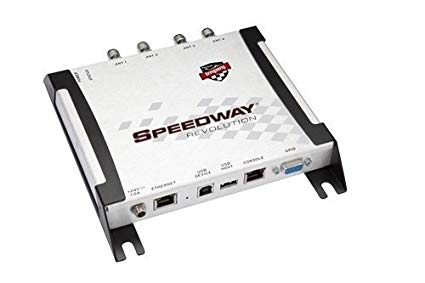
\includegraphics[width=0.8\linewidth]{figs/Metodologia/leitoraSpeedwayR420.jpg}
        \caption{Leitora Impinj Speedway R420 \cite{SpeedwayRUserManual}}
        \label{fig:SpeedwayR420_first}
    \end{figure}

 A leitora é capaz de registrar até 1100 etiquetas por segundo. Ela possui portas suficientes para o acoplamento de até 4 antenas, expansível até 32 antenas utilizando \textit{Hubs} específicos para esta aplicação. Dois protocolos são utilizados para a interface por ar: \textit{GS1/EPCglobal UHF Gen2 (ISO 18000-6C)} e \textit{RAIN RFID} \cite{SpeedwayRDatasheet}\cite{SpeedwayRUserManual}. As portas de conexão das antenas podem ser vistas na figura \ref{fig:SpeedwayR420front}.
 
     \begin{figure}[h]
        \centering
        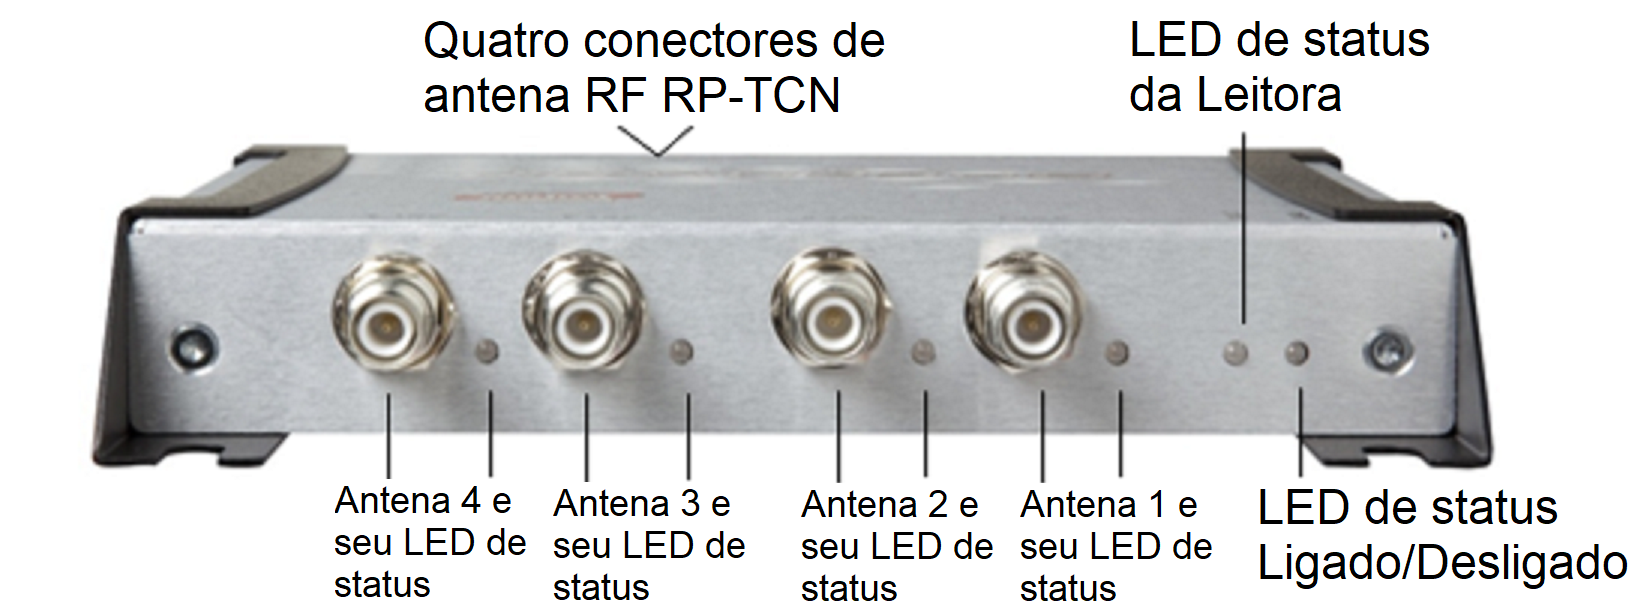
\includegraphics[width=0.8\linewidth]{figs/Metodologia/SpeedwayR420-front-view.png}
        \caption{Leitora Impinj Speedway R420 - vista frontal - Adaptado de \cite{SpeedwayRUserManual}.}
        \label{fig:SpeedwayR420front}
    \end{figure}
 
 Existem diversas portas na parte traseira da leitora Speedway R420. Uma delas é uma porta \textit{10/100 BaseT Ethernet} para comunicação em TCP/IP. A comunicação por TCP/IP é ideal para o uso comum, utilizando os softwares comercializados pela Impinj ou por programas feitos utilizando o pacote \textit{Impinj OctaneSDK}. Além dessa porta, a comunicação pode ser feita por USB ou por comunicação serial RS-232 em um conector RJ45 para acesso ao console embarcado na leitora. As portas seriais são ideais para utilização dos pacotes \textit{Impinj LTK} de programação em baixo nível, utilizando o padrão \textit{Low Level Reader Protocol} (LLRP). Baixo nível, neste caso, implica capacidade de alterar o protocolo de operação, o modo de marcação de tempo e dos parâmetros de comando por ar\cite{GS1-LLRP}\cite{SpeedwayRUserManual}. A visão traseira da leitora é apresentada na figura \ref{fig:SpeedwayR420back}.
 
\begin{figure}[h]
    \centering
    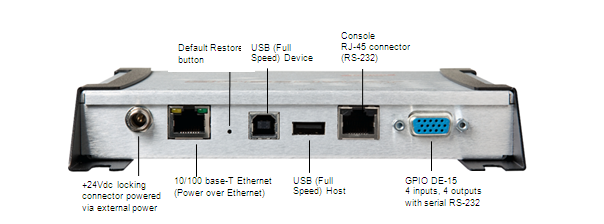
\includegraphics[width=0.9\linewidth]{figs/Metodologia/SpeedwayR420-back-view.png}
    \caption{Leitora Impinj Speedway R420 - vista traseira - Foto obtida no manual de instalação e operação da leitora - Adaptado de \cite{SpeedwayRUserManual}.}
    \label{fig:SpeedwayR420back}
\end{figure}
 
 Existe ainda uma porta \textit{GPIO DE-15} (\textit{General Purpose Input-Output DE-15} - Porta de uso de próstio geral para entrada e saída de dados)\cite{SpeedwayRUserManual}. Ela pode ser utilizada para a configuração de comandos e gatilhos de leitura.
 
 A alimentação elétrica da leitora pode ser feita utilizando o padrão \textit{PoE} (\textit{Power over Ethernet}) \cite{SpeedwayRUserManual}, ou seja, sem a necessidade de fonte externa, apenas através do cabo Ethernet, ou então pode ser feita com uma fonte 24 volts de corrente contínua \cite{IEEE-SA-POE}. A fonte pode prover uma confiabilidade maior para operação com potências maiores, próximas ao limite de 32,25 dBm, enquanto a alimentação \textit{PoE} permite maior flexibilidade na instalação do produto, principalmente em relação à passagem de cabos e instalação de tomadas.
 
 \subsubsection{Antena RFID Impinj Threshold}
 
 A Threshold, também da fabricante Impinj, é uma antena RAIN RFID específica para detectar cruzamento de barreiras e fronteiras. O seu corpo alongado, com polarização linear paralela ao menor eixo, permite uma ampla cobertura, e a possibilidade de conectar múltiplas antenas para criar uma "cortina" de cobertura RFID \cite{AntenaThresholdDatasheet}.A antena pode ser vista na figura \ref{fig:AntenaThreshold_first} a seguir.
 
 \begin{figure}[H]
    \centering
    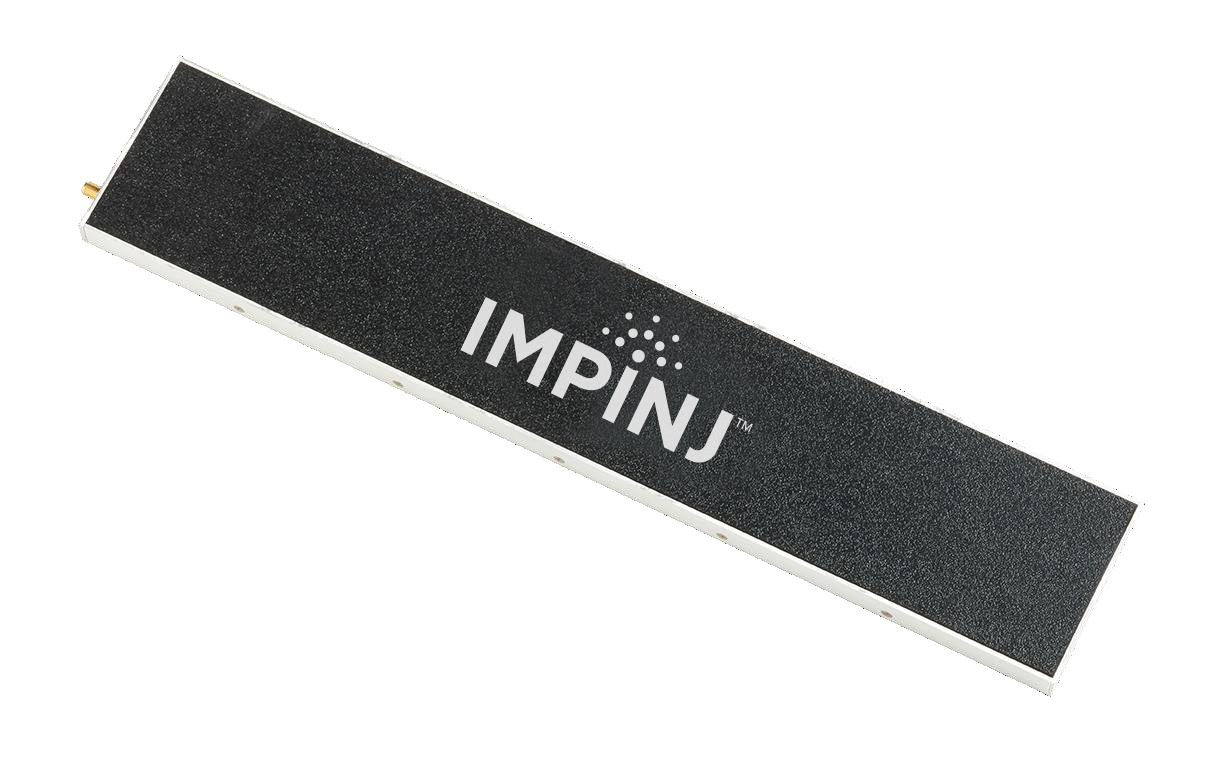
\includegraphics[width=0.6\linewidth]{figs/Metodologia/impinj_Threshold.png}
    \caption{Antena Impinj Threshold - Foto obtida no \textit{datasheet} da antena \cite{AntenaThresholdDatasheet}}
    \label{fig:AntenaThreshold_first}
\end{figure}
 
 A antena opera em duas faixas de frequência UHF: 902-928 MHz (FCC) e 865-868 MHz (ETSI), possui um ganho de campo distante de 5.0 dBi e impedância nominal de 50 $\Omega$ \cite{AntenaThresholdDatasheet}. A antena cobre um volume elipsoidal de dimensões 3m x 4m x 3m, como pode ser visto na figura \ref{fig:AntenaThresholdCobertura}.
 
  \begin{figure}[H]
    \centering
    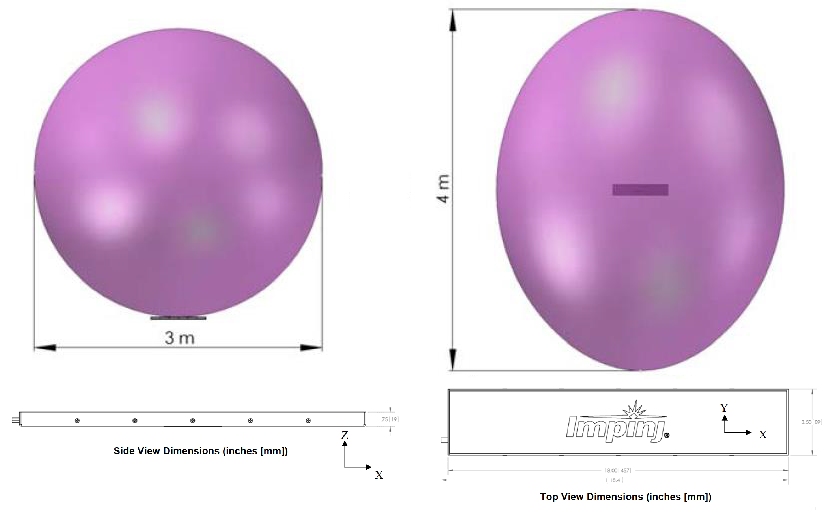
\includegraphics[width=0.6\linewidth]{figs/Metodologia/impinj_antenna_coverage.png}
    \caption{Gráfico da zona de cobertura das antenas Impinj Threshold e desenho mecânico da leitora em pontos de vista iguais aos dos desenhos de cobertura acima - Adaptado do \textit{datasheet} da antena \cite{AntenaThresholdDatasheet}}
    \label{fig:AntenaThresholdCobertura}
\end{figure}

\subsubsection{TAG utilizada no projeto}

As TAGs utilizadas são impressas em adesivos pela empresa Nycti BR. Elas utilizam chip Alien Higgs-3 RFID IC. Como características principais estão:

\begin{itemize}
    \item Banda de operação de 915-868 Mhz;
    \item Tamanho 96 X 23mm;
    \item Alcance de leitura de acordo com o fabricante de 6m (com testes empíricos feitos nas TAGs utilizadas de alcance de mais de 10m);
    \item 800-bit de memória, sendo 96 bits para armazenar o EPC - extensível até 480 bits - e 512 bits de uso de propósito geral; \cite{AlienHiggs3}
    \item ativado em baixíssimas potências de alimentação, ainda provendo excelente sinal de resposta de retroespalhamento. \cite{AlienHiggs3}
\end{itemize}

A figura \ref{fig:TAGsused} mostra as TAGs utilizadas para monitorar o trânsito das pessoas no interior dos ambientes pre-estabelecidos.

 \begin{figure}[H]
    \centering
    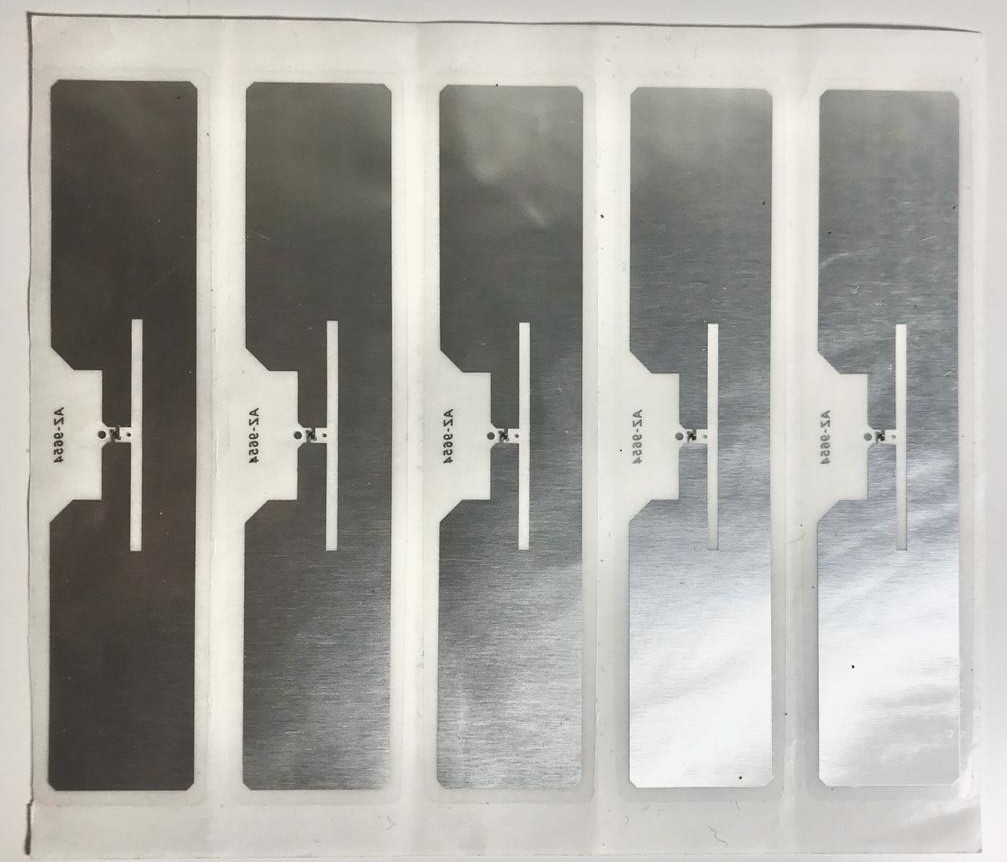
\includegraphics[width=0.8\linewidth]{figs/Metodologia/TAGsRFID.jpeg}
    \caption{TAGs utilizadas para a execução deste trabalho}
    \label{fig:TAGsused}
\end{figure}
 
 Estas TAGs mostradas na figura \ref{fig:TAGsused} foram distribuídas entre as pessoas designadas para testar o sistema criado. %TODO
 
 \subsubsection{Quantitativo}
 
 Este trabalho conta com leitoras e antenas RFID, além do espaço para trabalho e testes, gentilmente cedidos pelo Laboratório de Automação e Robótica (LARA) da UnB. No que se refere aos equipamentos, foram utilizados os seguintes dispositivos:
 
 \begin{itemize}
     \item 3 (três) Leitoras IMPINJ Speedway R420 (cedidas pelo LARA)
     \item 6 (seis) Antenas IMPINJ Treshold (cedidas pelo LARA)
     \item 1 (um) hub DLINK 6 portas Ethernet
     \item 20 (vinte) TAGs RFID 915 MHZ
     \item cabeamento e fontes de alimentação necessários
 \end{itemize}
 
 \subsection{Software} \label{section:met-software}
 
 Nesta parte do texto foram apresentadas as ferramentas computacionais utilizadas, suas características principais e como foram úteis na produção deste trabalho.
 
 \subsubsection{OctaneSDK}
 
 O pacote de desenvolvimento OctaneSDK para dispositivos RAIN RFID, da Impinj, foi utilizado para desenvolver a parte de software deste trabalho. O pacote possui versões para .NET e Java \cite{OctaneSDK}. O pacote para .NET foi lançado há mais tempo e possui mais versões, e, por conseguinte, mais defeitos foram corrigidos, o que torna esta implementação mais robusta do que o pacote em Java. Por esse motivo, foi escolhido para o desenvolvimento desse trabalho.
 
 \subsubsection{Visual Studio}
 
 O pacote OctaneSDK .NET foi desenvolvido para funcionar com o Ambiente Integral de Desenvolvimento (\textit{Integrated Development Environment} - IDE) Visual Studio, da Microsoft. A IDE foi utilizada para instalar o pacote de extensão do OctaneSDK. \cite{OctaneSDK}
 
 A linguagem de programação mais recomendada para desenvolvimento usando OctaneSDK com o Visual Studio é C\#. O desenvolvimento em outras linguagens baseadas em .NET \textit{framework} é possível, mas sem suporte da Impinj.

 
 \section{Abordagem utilizada} \label{abordagem}
 
 Três pontos foram essenciais para a execução deste trabalho: a instalação física das leitoras, antenas e demais equipamentos no local de teste; o \textit{software} de detecção de pessoas e cruzamento de fronteiras para a contagem de pessoas em um determinado ambiente;  e a elaboração de casos de teste para  validação da abordagem. Estes pontos serão descritos nas seções a seguir.
 
  
 \subsection{Instalação física}
 
 As leitoras e as antenas utilizadas neste trabalho possuem um grande campo de cobertura relativo a outros modelos de equipamentos RFID passivo. Entretanto, a cobertura de sinal anunciada pelo fabricante é válida para ambientes abertos e sem a presença de objetos que possam interferir no sinal, como: mesas, cadeiras, equipamentos e pessoas.
 
 A interferência de sinais de radiofrequência por metais e líquidos  é um problema conhecido na indústria. Levando em consideração este problema, um cenário fictício de um ambiente de trabalho é considerado, baseado em escritórios e laboratórios reais. Supõe-se que todos os trabalhadores e visitantes, carreguem consigo crachás de identificação, nos quais estão embutidos transpônderes RFID já existentes, utilizados no sistema de controle de acesso do escritório ou laboratório.
 
 As pessoas que transitam neste ambiente utilizam seus crachás em cordões dependurados no pescoço. Cada crachá permanece próximo ao corpo do seu usuário, porém não preso a ele. Os crachás ficam na altura do tórax.
 
 \subsection{O local} \label{section:local}
 

 O Laboratório de Automação e Robótica (LARA) foi o local para simulação do ambiente de teste do sistema criado, especificamente, a metade sul do laboratório, onde se encontram os ambientes de estudo geral e a sala de reuniões. A planta baixa do laboratório pode ser observada na figura \ref{fig:LARA_plata}.
 
   \begin{figure}[H]
    \centering
    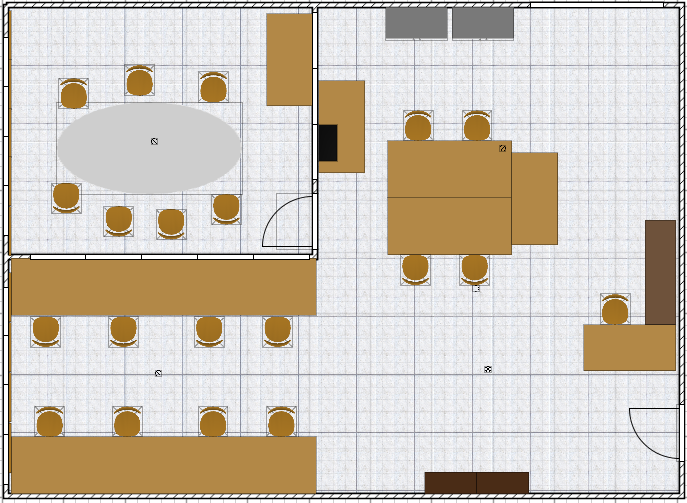
\includegraphics[width=0.7\linewidth]{figs/Metodologia/LARA_planta.PNG}
    \caption{Imagem apresentando a planta baixa do LARA}
    \label{fig:LARA_plata}
\end{figure}
 
 Esta parte do laboratório foi subdividida em quatro ambientes: o Ambiente Externo (0), a Sala Principal (1), Sala de Reuniões (2) e o Corredor de Baias (3), como apresentado na marcação sobre a planta baixa, na figura \ref{fig:LARA_planta}.

  \begin{figure}[H]
    \centering
    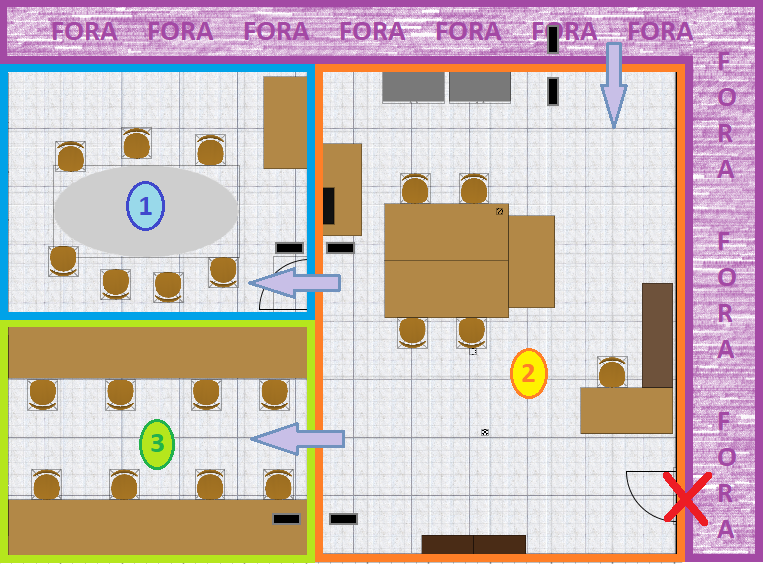
\includegraphics[width=0.7\linewidth]{figs/Metodologia/LARA_planta_ambientes.png}
    \caption{Imagem apresentando a planta baixa do LARA - local de instalação das leitoras}
    \label{fig:LARA_planta}
\end{figure}

O ambiente do laboratório pode ser melhor visualizado nas figuras \ref{fig:LARA1} e \ref{fig:LARA2}. As figuras mostram as projeções tridimensionais do laboratório, a partir de dois pontos de vista diferentes, para melhor compreensão do ambiente de estudo.

  \begin{figure}[H]
    \centering
    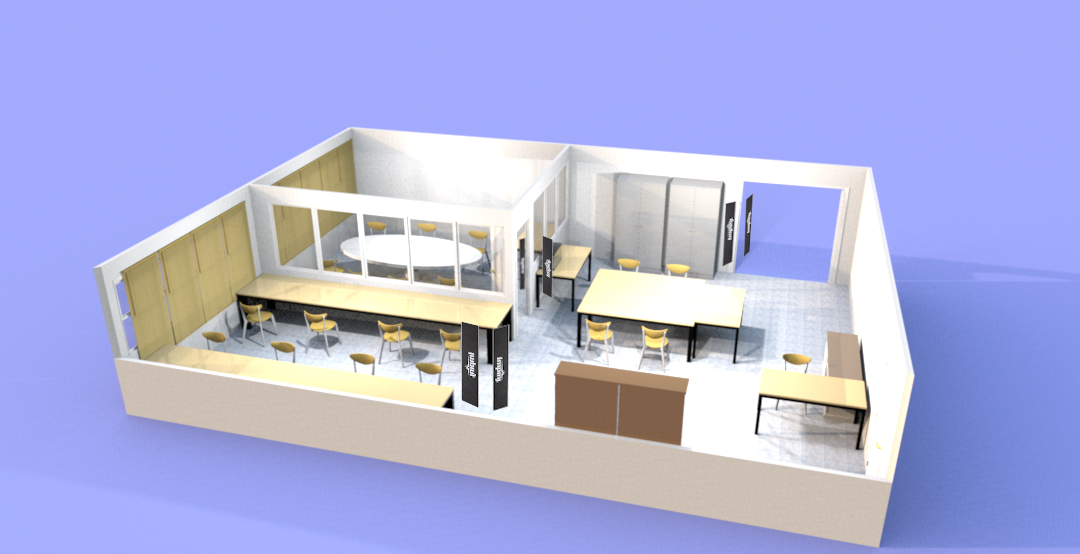
\includegraphics[width=1\linewidth]{figs/Metodologia/LARA_leitoras-1.png}
    \caption{Imagem apresentando a renderização tridimensional do LARA e o local de instalação das leitoras}
    \label{fig:LARA1}
\end{figure}

  \begin{figure}[H]
    \centering
    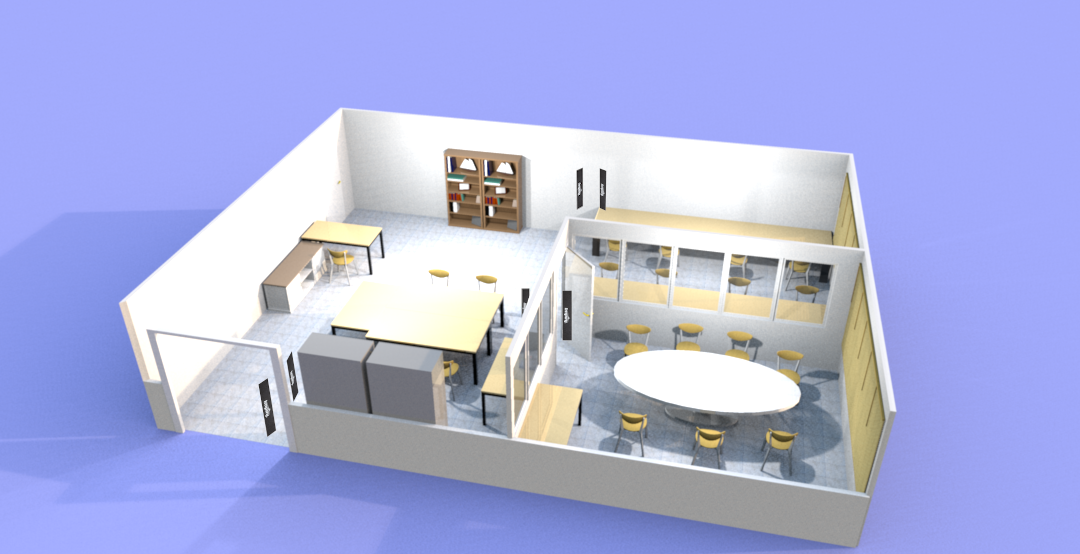
\includegraphics[width=1\linewidth]{figs/Metodologia/LARA_leitoras-2.png}
    \caption{Imagem apresentando a renderização tridimensional do LARA a partir de um segundo ponto de vista - local de instalação das leitoras}
    \label{fig:LARA2}
\end{figure}

As três leitoras foram designadas para tratar os dados das transições. A leitora 1 (L1) trata os dados da transição entre o Ambiente Externo (0) e a Sala Principal (1); a Leitora 2 (L2) é responsável por capturar os dados da transição entre a Sala Principal (1) e a Sala de Reuniões (2); a Leitora 3 registra os cartões que passam pela transição entre a Sala Principal (1) e o Corredor de Baias (3). Cada leitora é representada por um retângulo cinza na figura \ref{fig:LARA_planta} e possui duas antenas para registrar as TAGs que passam na região.

As antenas foram dispostas em locais estratégicos para se obter as leituras mais precisas, nos locais de transição de interesse. Estes locais estão localizados próximos às portas ou passagens onde estão as fronteiras dos ambientes definidos. As antenas podem ser vistas como retângulos pretos de borda cinza na figura \ref{fig:LARA_planta} e pelo desenho da leitora real nas figuras \ref{fig:LARA1} e \ref{fig:LARA1}.

As leitoras da transição entre os ambientes Sala Principal (1) e Sala de Reuniões (2) e da transição entre os ambientes Sala Principal (1), Corredor de Baias (3) foram instaladas em posições opostas da sala para minimizar a ocorrência de leitura das TAGs pelas duas leitoras ao mesmo tempo. A marcação feita sobre a planta baixa, apresentada na figura \ref{fig:LARA_planta}, mostra em laranja, uma elipse estimando o alcance do campo de leituras da interrogadora L1, em azul, da leitora L2 e, em verde, a elipse de alcance da leitora L3. 

 \subsection{Elaboração do \textit{Software}} \label{section:software}
 
 A tecnologia RAIN RFID, geralmente utilizada para aplicações de \textit{IoT} (Internet das coisas - \textit{Internet of Things} em inglês), exige a implementação de um \textit{middleware} para conectar os dados crus das TAGs registrados pelas leitoras RFID às aplicações de alto nível e de computação em nuvem, como pode ser observado na figura \ref{fig:RFID-Middleware} do capítulo anterior, seção \ref{section: middleware}. Por esse motivo, o pacote OctaneSDK da Impinj foi escolhido para implementar a aplicação de localização de pessoas. O pacote possui classes prontas de comunicação e configuração das leitoras Impinj Speedway R420 usadas. Será considerado, portanto, que o programa criado não se trata de um \textit{middleware}, mas de uma aplicação apenas, mesmo executando tarefas de comunicação com as leitoras.
 
 O \textit{software} elaborado simula internamente o ambiente do LARA como uma Rede de Petri, onde cada estado da rede representa um ambiente do LARA enquanto cada transição representa um par de antenas instaladas nas portas ou passagens. Os marcadores da Rede de Petri representam as TAGs das pessoas, transitando livremente pelos ambientes e transições. Um modelo que representa o funcionamento do programa pode ser visto na figura \ref{fig:Petri1}.
 
 \begin{figure}[h]
    \centering
    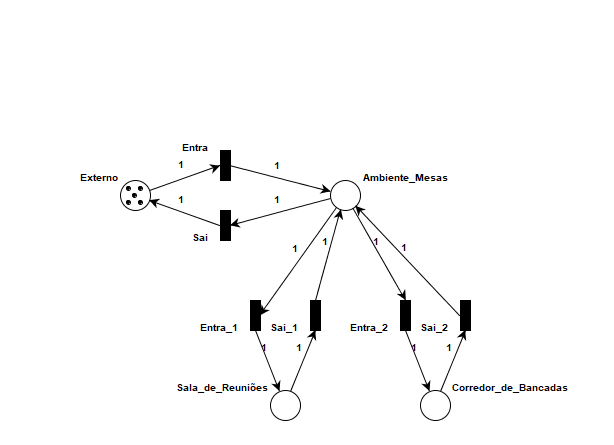
\includegraphics[width=0.8\linewidth]{figs/Metodologia/Petri_net.png}
    \caption{Rede de Petri representando todas as possibilidades circulação de pessoas pelo LARA como estados e transições}
    \label{fig:Petri1}
\end{figure}

Simulando a Rede de Petri é possível observar a ideia da circulação das pessoas pelo espaço do laboratório, onde cada transição ativada leva um marcador de um estado a outro, o que corresponde a uma pessoa cruzando uma fronteira para ir de um ambiente a outro. A figura \ref{fig:Petri2} mostra uma situação imaginária onde cinco pessoas transitam pelo laboratório. As transições marcadas em vermelho são as transições possíveis a partir do estado atual. A situação apresentada mostra duas pessoas na Sala Principal (1), duas pessoas na Sala de Reuniões (2) e uma pessoa no Corredor de Baias (3).

 \begin{figure}[h]
    \centering
    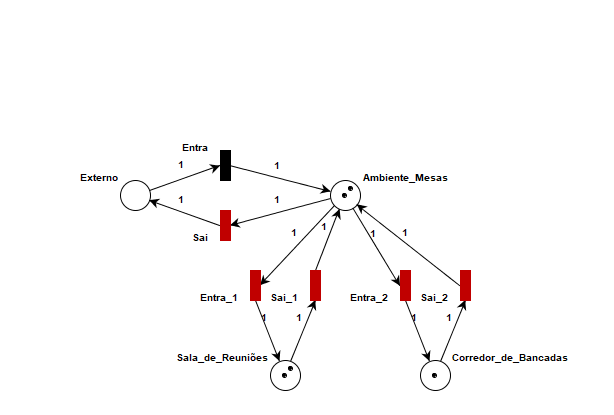
\includegraphics[width=0.8\linewidth]{figs/Metodologia/Petri_net2.png}
    \caption{Rede de Petri representando a circulação de pessoas pelo LARA em um caso hipotético}
    \label{fig:Petri2}
\end{figure}
 
 Os números próximos a cada seta entre um estado e uma transição nas figuras \ref{fig:Petri1} e \ref{fig:Petri2}, neste caso todos iguais a $1$, mostram o peso de cada transição. Dessa forma, a rede de Petri apresentada nas figuras possui igual probabilidade do acionamento de cada transição. A rede não necessariamente precisa ser implementada com uma entrada e uma saída para cada estado. É possível encadear sequências em série, como o trajeto $"externo" \rightarrow "entra" \rightarrow "ambiente\_mesas" \rightarrow "entra\_1" \rightarrow "sala\_ de\_ reunioes"$.
 
 O programa criado em linguagem de programação C\# é orientado a objeto e cria as seguintes classes:
 
 \begin{itemize}
     \item \textbf{Programa:} contém a função \textit{main} e as funções básicas de configuração, comunicação e leituras;
     \item \textbf{Ambiente:} possui um nome, pode ter pessoas (\textit{cardholders}) e possui uma carga térmica associada à quantidade de pessoas em seu interior;
     \item \textbf{Pessoa (\textit{Cardholder}):} possui um nome, uma TAG (o número EPC associado à TAG) e uma carga térmica. Guarda a informação do ambiente em que se encontra e das curvas de histórico de leituras de valores RSSI e frequência Doppler;
     \item \textbf{Curva:} armazena os últimos $n$ valores de RSSI ou frequência Doppler, assim como o horário das leituras em que se capturaram essas informações;
     \item \textbf{Antena:} possui um número e está associada a uma leitora;
     \item \textbf{Transição:} conecta dois ambientes, e monitora duas antenas;
     \item \textbf{Projeto:} implementa os critérios de decisão de transição e registra as mudanças de ambiente dos \textit{cardholders};
     \item \textbf{Gerenciador de arquivos (\textit{FileHandler}):} Organiza e registra os dados coletados em arquivos CSV.
 \end{itemize}
 
 \subsection{Configuração das Leitoras}

  A correta configuração das leitoras é provavelmente a parte mais importante deste trabalho. O estudo cuidadoso de todos os modos de operação possíveis, observando o manual do fabricante \cite{SpeedwayRUserManual}, \textit{datasheet} das leitoras \cite{SpeedwayRDatasheet} e guias de programação e códigos de exemplo \cite{OctaneSDK} resultou na escolha dos parâmetros apresentados nesta seção.
  
  Primeiramente, conecta-se à cada leitora. Para isso, é necessário informar o caminho de rede para realizar a conexão. As leitoras foram configuradas com IP (\textit{Internet Protocol}) fixo, em uma rede local fechada. O uso de uma rede local simplifica o comissionamento dos equipamentos e torna o sistema de localização de pessoas um pouco mais seguro, visto que RFID passivo é uma tecnologia muito suscetível a ataques à privacidade dos usuários e ataques destrutivos, como mostra Juels \textit{et al.} \cite{juels2006rfid}. Para acessar as leitoras, o nome padrão de domínio DNS (Sistema de Nomes de Domínio - em inglês \textit{Domain Name System}) foi utilizado para facilitar a identificação das leitoras. O domínio DNS padrão das leitoras é composto pelo modelo, seguido dos três últimos pares de dígitos do número de série de cada uma, que estão impressos em etiquetas coladas a cada uma.

  A figura \ref{fig:set_readers} mostra a configuração dos caminhos de rede e a nomeação das leitoras. Através dos métodos \textit{"new"} e \textit{"Add"}, os objetos de cada leitora são criados e armazenados na classe \textit{"readers"}.

 \begin{figure}[H]
    \centering
    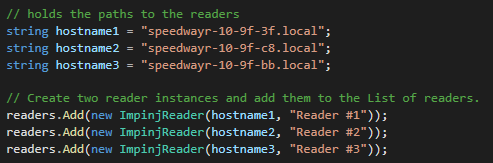
\includegraphics[width=0.8\linewidth]{figs/Metodologia/set_readers.PNG}
    \caption{Comandos de linha de código para estabelecer as leitoras}
    \label{fig:set_readers}
\end{figure}

 Em seguida, a primeira ação a ser executada é a criação do mapa da sala, com ambientes e transições, como discutido nas sessões \ref{section:local} e \ref{section:software}. Os ambientes criados são "Area\_Externa(0)", "Sala\_Principal(1)", "Sala\_Reuniao(2)" e "Corredor\_Baias(3)". As transições 1, 2 e 3 são criadas e associadas às respectivas leitoras e antenas, conforme montado fisicamente no laboratório. A implementação pode ser vista na figura \ref{fig:set_AmbTran}.

 \begin{figure}[H]
    \centering
    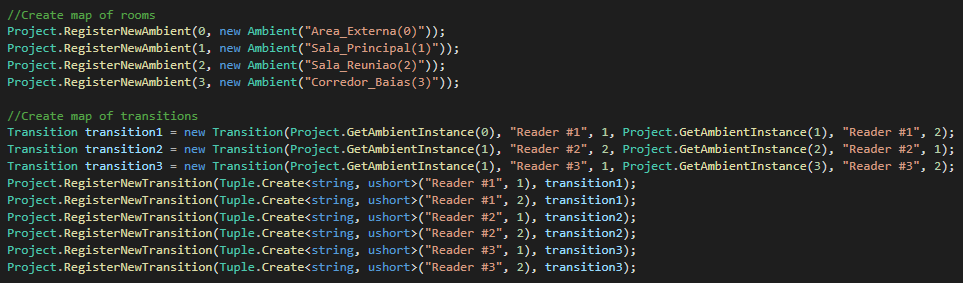
\includegraphics[width=1\linewidth]{figs/Metodologia/set_rooms&transitions.PNG}
    \caption{Comandos de linha de código para estabelecer os ambientes e as transições}
    \label{fig:set_AmbTran}
\end{figure}

  A principal função da leitora RFID é reportar as informações coletadas do campo. A figura \ref{fig:report_settings} mostra as configurações de \textit{report} feitas. As informações coletadas em cada leitura incluem: qual antena coletou a informação, o horário em que a TAG foi vista a primeira e a última vez (em cada \textit{report}), a quantidade de vezes que a TAG foi vista (em cada \textit{report}), a frequência Doppler e o pico de potência RSSI da leitura. 
  
  O modo de \textit{report} escolhido foi o modo individual, ou seja, a leitora envia um relatório a cada TAG lida. Isso inutiliza algumas funções nativas das leitoras, como os horários em que a TAG foi vista a primeira e a última vez e a quantidade de vezes que a TAG foi vista, mas possibilita a operação em tempo real (em um sentido mais amplo, não estritamente rígido), que é essencial para a aplicação criada neste trabalho.

 \begin{figure}[H]
    \centering
    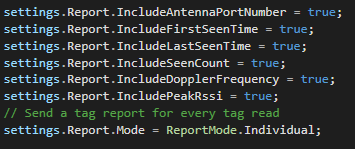
\includegraphics[width=0.6\linewidth]{figs/Metodologia/report_settings.PNG}
    \caption{Comandos de linha de código para configurar o modo de \textit{report} das leitoras}
    \label{fig:report_settings}
\end{figure}

 Após a configuração das leitoras, é necessário configurar as antenas (na realidade são as leitoras que são ajustadas nesta etapa, visto que as antenas são elementos passivos e fixos, mas os parâmetros alterados nesta parte são referentes ao funcionamento das antenas). Primeiramente são apagadas as configurações padrão e duas antenas são ativadas manualmente em cada leitora com potência máxima e sensitividade máxima. Existe a possibilidade de programar as leitoras para identificarem novas antenas automaticamente, todavia, para esta aplicação, onde a quantidade de antenas é fixa, não é necessário ativar essa função. O procedimento pode ser visto na figura \ref{fig:antenna_settings}.

 \begin{figure}[H]
    \centering
    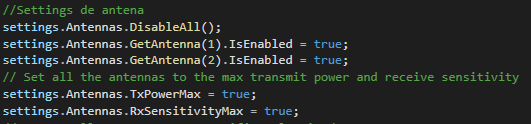
\includegraphics[width=0.8\linewidth]{figs/Metodologia/antenna_settings.PNG}
    \caption{Comandos de linha de código para configurar o modo de operação das antenas}
    \label{fig:antenna_settings}
\end{figure}

  Finalmente, uma última função é ativada: o modo de leitura dos equipamentos é alterado para \textit{"DenseReaderM8"}. Este modo ativa parâmetros internos da leitora para prover a maior quantidade de leituras com a maior confiabilidade possível. Este modo é modo de funcionamento mais lento, que provê leituras escassas, mas confiáveis. Ao ativar esse modo, boa parte das leituras devido a reflexão e falsas leituras são filtradas em \textit{hardware}. O comando pode ser visto na figura \ref{fig:readermode_settings}.

 \begin{figure}[H]
    \centering
    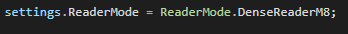
\includegraphics[width=0.6\linewidth]{figs/Metodologia/readermode_settings.PNG}
    \caption{Comando de linha de código para configurar o modo de operação das leitoras}
    \label{fig:readermode_settings}
\end{figure}

  Após as configurações, as leitoras são iniciadas, uma \textit{tread} de leitura e uma de processamento de dados são abertas, e as configurações estão finalizadas.

\section{Taxa de amostragem} \label{section:amostragem}

A partir da equação \ref{eq:taxadeamostragem}, calcula-se:

\begin{equation}
    T_A = \frac{1}{900.000.000}*8*800*1 = 0,000007 = 7\mu s
    \label{eq:amostragem2}
\end{equation}

Na equação \ref{eq:amostragem2} considerou-se $M=8$, pois o modo de leitura utilizado neste trabalho foi \textit{"DenseReaderM8"}. A quantidade de Bits presentes na TAG utilizazda é $800$. A interferência de múltiplas TAGs foi definida como $1$, para que se calcule o período de amostragem mínimo. Isso resultou em $T_A = 7 \mu s$.

Apesar dos cálculos, empiricamente, que somando os atrasos do \textit{software} interno da Leitora, do \textit{software} desenvolvido neste programa, das comunicações via \textit{Ethernet} e dos casos onde múltiplas TAGs são lidas ao mesmo tempo (caso onde 20 TAGs chegam a atrasar a leitura em até 10 vezes o período normal para a leitura de cada TAG), o período de amostragem de TAGs em situações ideais fica entre $1 ms$ e $30 ms$.

Entretando, considerando ainda as obstruções de sinal do meio físico, a água no corpo do usuário do cartão, as múltiplas superfícies de reflexão do ambiente fechado do LARA e a interferência de sinal com as outras TAGs, antenas, demais fontes de sinal UHF do laboratório e com o próprio sinal de cada TAG refletido nas paredes, chão e teto, o período de amostragem real pode chegar a superar $1$s entre uma leitura e outra.


 \subsection{Transições}
 
 Com o intuito de definir com a maior precisão possível o momento de passagem de uma pessoa de um ambiente para outro foi decidido monitorar as portas e passagens com duas antenas. O objetivo é acumular dados de potência de \textit{backscattering} das TAGs (RSSI) para possuir um valor comparativo de proximidade da TAG para cada antena. Além do sinal de potência RSSI, também é coletada a frequência de efeito Doppler, que indica um valor proporcional a velocidade vetorial em direção ortogonal à leitora, e pode indicar se a pessoa se aproxima ou de afasta desta.
 
 Durante testes preliminares, o analisou-se a variação dos valores de RSSI e frequência Doppler com uma única TAG e uma única antena. Os resultados deste teste podem ser encontrados na seção \ref{sect:testepreliminar}. Com base nesses resultados duas conclusões foram tiradas: as leituras de frequência de efeito Doppler podem ser facilmente divididas entre aproximação e afastamento de uma determinada antena e as leituras de potência RSSI aumentam proporcionalmente com a proximidade da TAG à antena, e diminuem proporcionalmente ao afastamento.
 
 A partir dessa ideia foi criado o conceito de transição, onde duas antenas registram a passagem de uma pessoa, e comparam entre si os dados RSSI e de frequência Doppler para estimar o sentido do caminhar da pessoa (entrando ou saindo de um ambiente). Cada antena fica de um lado da fronteira (porta ou passagem).
 
 Definindo-se o maior valor de RSSI durante todas as leituras na passagem de uma pessoa por uma fronteira, define-se esse como o momento em que a pessoa está mais próxima daquela antena. Realiza-se o mesmo procedimento para a segunda antena, do outro lado da fronteira. O ponto médio define o momento de transição de um ambiente para o outro. Da mesma forma, o momento em que uma pessoa deixa de aproximar-se e passa a se afastar de uma antena, este é o momento em que a pessoa está mais próxima da antena. Utilizando o mesmo critério do RSSI, o ponto médio entre o cruzamento na frente das duas antenas marca o momento de transição.
 
 \subsubsection{Curvas} \label{section:curvas}
 
 Foram criados dois \textit{buffers} para armazenar as últimas leituras de cada TAG. Cada um armazena uma lista ordenada de tuplas $<x,y>$, onde $x$ é o tempo da leitura, e $y$ é a magnitude. A lista é ordenada com base na chave $x$, para garantir que os dados são salvos em ordem cronológica. O primeiro \textit{buffer} armazena as leituras de RSSI. O segundo armazena as leituras de frequência Doppler.Os \textit{buffers} foram chamados de "curvas", por guardarem as curvas históricas das últimas $n$ leituras para cada valor.
 
 O tamanho das curvas, inicialmente foi definido em 100 valores. Este se mostrou um valor demasiado grande, pois armazena dados de mais de uma passagem anterior, e atrapalha a análise dos dados. Definiu-se então que as curvas armazenariam 5 a 20 valores, padronizado em 12 leituras, por ser a faixa do tamanho médio da quantidade de leituras feitas em uma passagem a passos curtos em velocidade constante na frente das antenas.
 
 Após encher o \textit{buffer}, cada próxima leitura será armazenada no final da lista, após a retirada do primeiro elemento, tornando o \textit{buffer} uma fila.

 
 \subsection{Estratégias e casos de teste} \label{section:estrategias}

 Durante a fase de planejamento deste trabalho, inicialmente foi cogitado o uso de apenas uma leitora por transição, utilizando apenas as informações fornecidas pelas leitoras de potência de retorno do sinal das TAGs (RSSI) e frequência de efeito Doppler para definição da posição de uma TAG em um ambiente ou outro. Essa ideia foi promissora em um primeiro momento, e chegou a mostrar bons resultados, como pode ser visto na seção \ref{sect:testepreliminar}. A identificação de um cruzamento de fronteira era feita corretamente na maioria das vezes, e as leituras geralmente produziam dados suficientes para a correta identificação da transição.
 
 Entretanto, o problema com esta estratégia é que no momento em que adicionam-se ambientes vizinhos, com outras leitoras e outras antenas próximas, pessoas circulando e uma quantidade maior de TAGs, começam a surgir leituras erradas nas zonas de transição. Por exemplo: No ambiente do LARA, ao realizar o monitoramento com apenas uma antena na transição entre a Sala Principal (1) e a Sala de Reuniões (2), e uma antena na transição entre a Sala Principal (1) e o Corredor de Baias (3), no momento em que se passa por uma, leituras também são captadas pela outra. 
 
 Devido aos caminhos múltiplos que os sinais RF podem tomar em um ambiente fechado devido à reflexão (do chão, teto, paredes e objetos próximos, como mesas, cadeiras, hastes de metal, equipamentos, etc.), a leitura de potência RSSI pode ser enganosa e mostrar a transição em um ambiente, quando na verdade se encontra em outro. Além disso, ao ficar próximo de uma divisória, como a parede da Sala de Reuniões (2), em alguns casos, sinais podem ser captados em antenas de fora da sala, enganando o programa e registrando uma troca de sala para outro ambiente. Por esse motivo, uma topologia similar à usada em sistemas de gerenciamento de estoque e sistemas  controle de carga e descarga de caminhões \cite{PortalRFID} foi considerada como uma alternativa mais robusta do que apenas a detecção da presença de uma TAG.
 
 Disponibilizando duas antenas para cada transição, é possível obter informações mais confiáveis de leitura, e ainda possui a vantagem de saber o sentido da travessia. Dessa forma, diminui-se o risco de registrar a entrada ou saída de uma pessoa em um ambiente apenas por registrar leituras de proximidade a uma antena. As antenas foram posicionadas de maneira similar à observada na figura \ref{fig:antenas1}. Esta foto, apesar de não ser o local final, permite a visualização da orientação e espaçamento das antenas para registrar a travessia de uma pessoa em sua frente. As leitoras e antenas, instaladas em seu local definitivo, podem ser visualizadas nas figuras \ref{fig:cruzamento01}, \ref{fig:cruzamento10}, \ref{fig:cruzamento12}, \ref{fig:cruzamento21}, \ref{fig:cruzamento13} e \ref{fig:cruzamento31}.
 
  \begin{figure}[H]
    \centering
    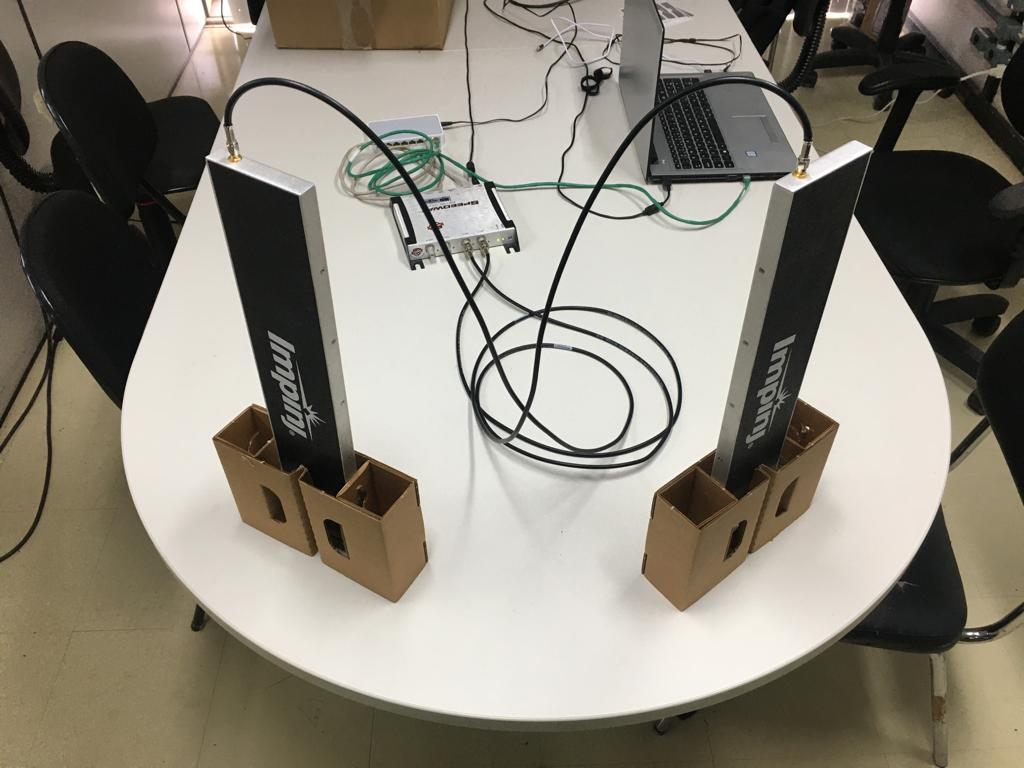
\includegraphics[width=0.6\linewidth]{figs/Metodologia/antenas1.jpeg}
    \caption{Montagem das antenas em local provisório. É possível visualizar a orientação e distanciamento das antenas.}
    \label{fig:antenas1}
\end{figure}
 
 Foram elaboradas duas ideias principais, que foram estendidas para seis, ao final do estudo. As duas principais são discutidas nas sessões \ref{section:picos_met} e \ref{section:doppler_met}, e as demais (sessões \ref{section:ultimo_valor_met}, \ref{section:RSSI+doppler_met}, \ref{section:mean_met} e \ref{section:median_met}) são derivadas das suas primeiras.

 \subsubsection{Comparando a magnitude do último valor de RSSI capturado} \label{section:ultimo_valor_met}
 
 Iniciando pela ideia mais simples: comparam-se as últimas leituras em ambas as antenas. O princípio é utilizar a informação de potência do sinal de retorno das TAGs para a leitora, o sinal RSSI, como indicador de proximidade de uma antena. Quanto mais próximo uma TAG está de uma antena, maior é o sinal RSSI registrado. Quanto mais distante uma TAG está da antena, menor é o sinal. Testes com as TAGs utilizadas no projeto mostraram que, quando estão rentes às antenas, encostando nelas, o sinal RSSI registrado chega a ser maior que $-30dB$. Ao afastar a TAG da antena, com a face da etiqueta apontando para ela, na orientação mais favorável à leitura pela antena (devido à polarização do sinal), o sinal mais fraco registrado foi ligeiramente menor que $-70dB$. O fabricante indica que as antenas são capazes de registrar até $-90dB$ de sinal de retorno RSSI, mas com as TAGs utilizadas e em um ambiente poluído para aplicações de RF uma leitura tão fraca não existiu.
 
 Considerando que uma pessoa passe em frente às leitoras da foto \ref{fig:antenas1} da direita para a esquerda, ou da esquerda para a direita, comparando-se o valor da magnitude da última leitura RSSI, em teoria, o valor lido pela antena mais próxima será sempre o mais forte. Como as duas antenas estão próximas, durante a maioria das leituras as duas antenas enxergarão a TAG a sua frente.
 
 \begin{figure}[H]
    \centering
    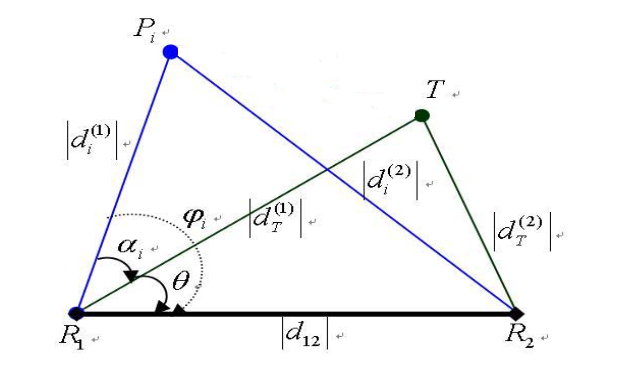
\includegraphics[width=0.8\linewidth]{figs/Metodologia/maisproxima.PNG}
    \caption{Esquemático das distâncias das TAGs às antenas (adaptado de Bekkali \cite{bekkali2007rfid}}
    \label{fig:maisproxima}
\end{figure}
 
  A figura \ref{fig:maisproxima} mostra duas posições $P$ e $T$, que representam duas posições possíveis para uma TAG em frente às antenas $R_1$ e $R_2$. Como a distância de $P$ para $R_2$ é maior que de $P$ para $R_1$, o sinal RSSI será mais forte em $R_1$. Já $T$ está mais próximo de $R_2$, e portanto o seu sinal RSSI será mais forte em $R_2$ do que em $R_1$.

 \subsubsection{Comparando o tempo dos últimos picos das curvas de RSSI} \label{section:picos_met}
 
 Aprimorando a ideia da seção \ref{section:ultimo_valor_met}, caso o valor das últimas leituras das antenas seja armazenado, mais informações podem ser obtidas do que apenas a proximidade instantânea das antenas.
 
 Criando curvas que armazenam esses valores, como discutido na seção \ref{section:curvas}, é possível analisar toda a trajetória da pessoa em frente às antenas. Utilizando as curvas fictícias das figuras \ref{fig:rssicurvesmet1} e \ref{fig:rssicurvesmet2}, é possível explicar a ideia da comparação de picos.
 
\begin{figure}[H]
    \centering
    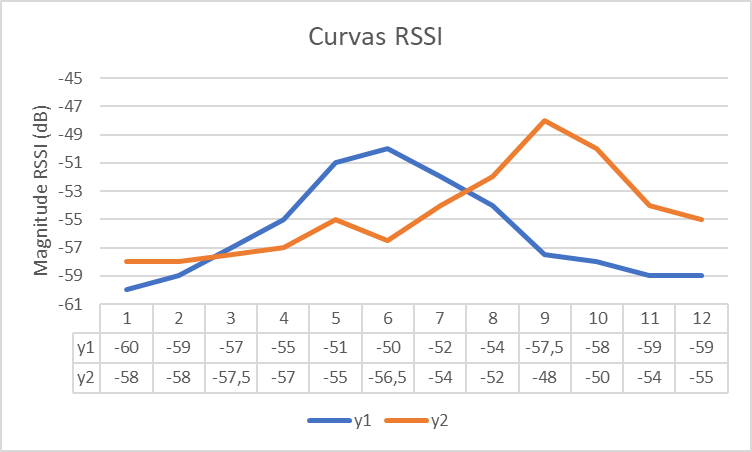
\includegraphics[width=0.8\linewidth]{figs/Metodologia/image001.png}
    \caption{Exemplo de curvas RSSI com dados gerados artificialmente}
    \label{fig:rssicurvesmet1}
\end{figure}


 Supondo que uma pessoa portando uma etiqueta RFID em seu crachá caminhe em frente às leitoras da figura \ref{fig:antenas1}. Definimos a antena da esquerda como a antena $y_1$, e a antena da direita como $y_2$. Ao caminhar da esquerda para a direita, a pessoa passa primeiramente em frente à antena $y_1$, e em seguida passa em frente à antena $y_2$. A cada período de tempo $x$ - onde nesse caso teórico não atribuímos um valor de tempo definido para $x$ a fim de facilitar o entendimento, apenas números inteiros de 1 a 12 - registra-se o valor de potência RSSI para a mesma TAG nas duas antenas nas curvas da figura \ref{fig:rssicurvesmet1}, $y_1$ em azul e $y_2$ em laranja. Os tempos $x$ de 1 a 12 mostram a progressão no tempo.
 
 \begin{figure}[h]
    \centering
    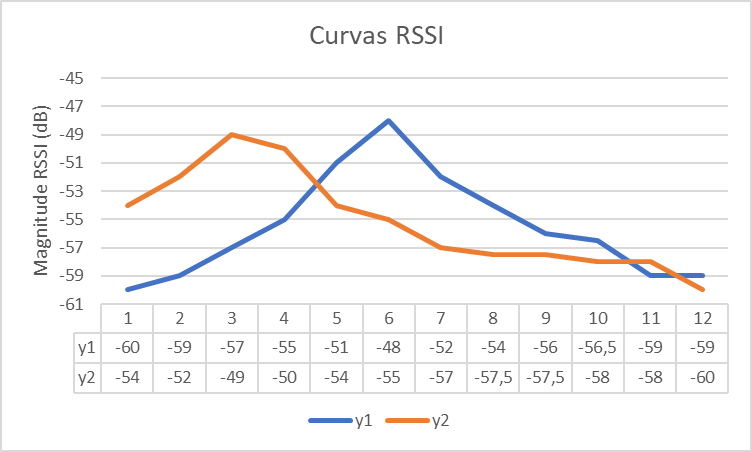
\includegraphics[width=0.8\linewidth]{figs/Metodologia/image005.png}
    \caption{Exemplo de curvas RSSI com dados gerados artificialmente}
    \label{fig:rssicurvesmet2}
\end{figure}
 
 É possível perceber que entre os tempos $x=5$ e $x=7$ existe a maior probabilidade de a pessoa estar em frente à antena $y_1$, pois esse trecho apresenta os valores máximos de RSSI para essa antena. Entre os períodos $x=8$ e $x=10$ existe a maior probabilidade de a pessoa estar em frente à antena $y_2$, pois esse trecho apresenta os valores máximos de RSSI para essa antena. Já as curvas da figura \ref{fig:rssicurvesmet2} mostram o oposto: entre os períodos $x=2$ e $x=4$ a pessoa provavelmente passa em frente à antena $y_2$ e de $x=5$ a $x=7$ em frente à antena $y_1$.
 
 A partir dessa informação, conclui-se que na situação da figura \ref{fig:rssicurvesmet1} a pessoa caminha da direita para a esquerda, em frente às leitoras. Já na figura \ref{fig:rssicurvesmet2}, a pessoa caminha da esquerda para a direita. O intervalo entre o pico das duas curvas é o trecho entre as duas antenas. Define-se o ponto médio entre os dois picos como o ponto de cruzamento.
 
  \begin{figure}[h]
    \centering
    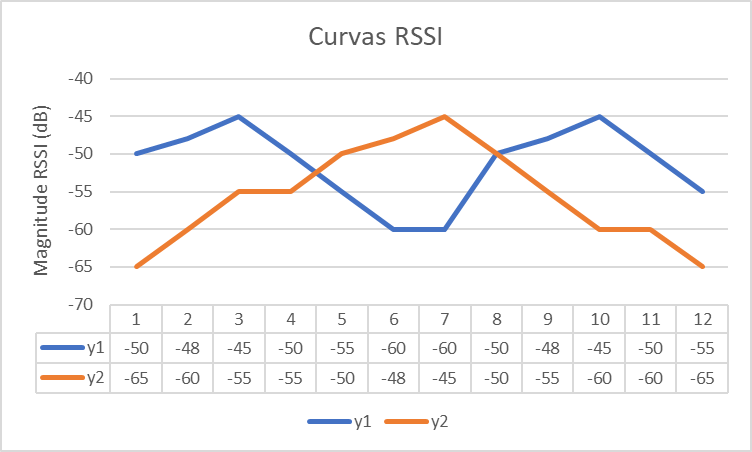
\includegraphics[width=0.8\linewidth]{figs/Metodologia/curvas1.png}
    \caption{Exemplo de curvas RSSI com dados gerados artificialmente}
    \label{fig:rssicurvesmet3}
\end{figure}

Um caso mais complicado onde a pessoa volta para o caminho de onde veio é mostrado na figura \ref{fig:rssicurvesmet3}, também gerada com dados artificiais. Neste caso, dois picos são criados na curva azul, da antena $y_1$. Para tratar este tipo de imprevisto, o método da comparação dos tempos de pico também é robusto. Comparando os picos mais recentes, apenas, o critério de decisão enxergará um pico de potência RSSI de $y_2$ em $x=6$ e um pico de potência RSSI de $y_1$ em $x=10$, definindo o ambiente onde a pessoa está como o lado da antena $y_1$, ou seja, no lado correto.
 
\subsubsection{Comparando a média das curvas de potência RSSI} \label{section:mean_met}

 Dado que se possui um \textit{buffer} repleto dos últimos dados de potência RSSI, obtidos pelas curvas armazenadas, considera-se a ideia de que a média desses valores possa indicar o lado da antena mais próxima. Estima-se que as últimas coletas de valores de RSSI na antena mais próxima, maiores que os da antena adjacente, possam fornecer bons indicadores de qual ambiente a pessoa ocupa.
 
 A figura \ref{fig:mediamediana_met} mostra um comparativo entre duas curvas e suas médias, em uma situação hipotética onde uma pessoa permanece mais próxima da antena $y_1$ do que da antena $y_2$ por tempo suficiente para que as leituras de dados de RSSI preencham toda a curva.

\subsubsection{Combinando a mediana das curvas de potência RSSI} \label{section:median_met}
 
 Da mesma forma, aproveitando os dados das curvas, estima-se que a mediana dos dados seja maior do lado onde os últimos registros de leitura de TAG sejam feitos.
 
  A figura \ref{fig:mediamediana_met} mostra um comparativo entre duas curvas e suas medianas, assim como as médias. O valor das medianas geralmente é diferente, mas não muito distante do valor das médias.

   \begin{figure}[H]
    \centering
    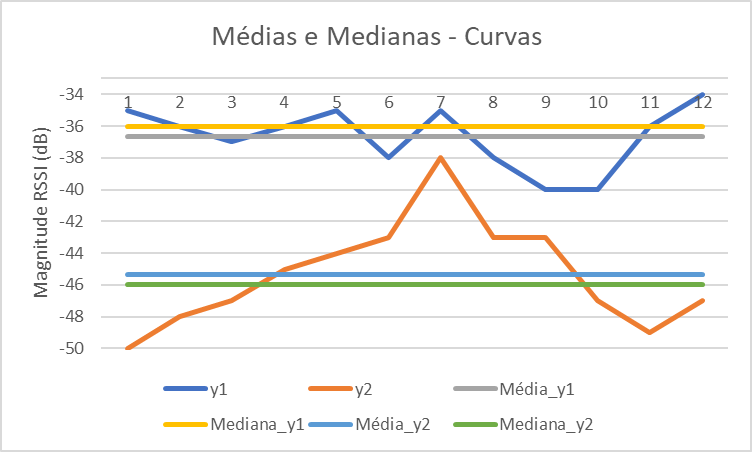
\includegraphics[width=0.8\linewidth]{figs/Metodologia/mediamediana.png}
    \caption{Exemplo de curvas RSSI com dados gerados artificialmente para cálculo de médias e medianas das curvas}
    \label{fig:mediamediana_met}
\end{figure}
 

 \subsubsection{Utilizando o Efeito Doppler como critério de travessia} \label{section:doppler_met}
 
  O outro dado relevante para utilização como critério de rastreamento de pessoas é a frequência Doppler. Os dados fornecidos pelas leitoras indicam um número proporcional à componente de velocidade vetorial ortogonal à antena, como visto na seção \ref{section:doppler_fund}. A figura \ref{fig:doppler_MET} mostra dados gerados artificialmente de frequência Doppler simulando uma pessoa caminhando em velocidade constante em frente às antenas.
 
   \begin{figure}[H]
    \centering
    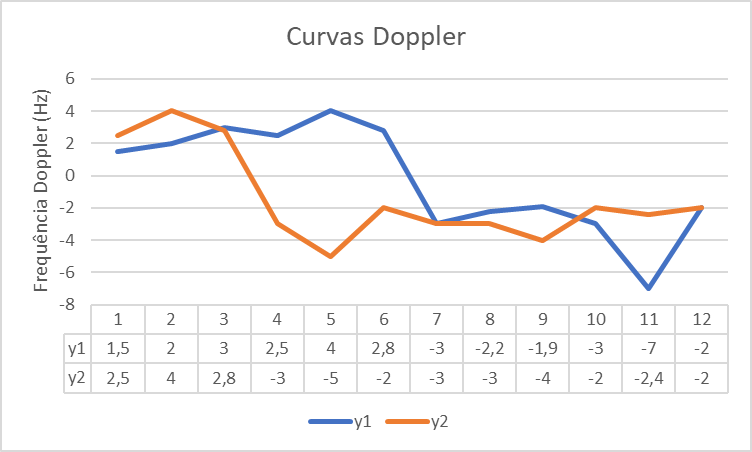
\includegraphics[width=0.8\linewidth]{figs/Metodologia/image003.png}
    \caption{Exemplo de curvas Doppler com dados gerados artificialmente}
    \label{fig:doppler_MET}
\end{figure}

    Os dados fornecidos pela leitora, geralmente ficam na faixa entre $\pm 10 Hz$. Valores maiores que zero indicam aproximação enquanto valores menores que zero indicam afastamento. Utilizando a equação \ref{eq:dopplerNorm} é possível normalizar os dados entre $1$ e $-1$, criando um sinal binário (positivo ou negativo). A normalização dá origem à figura \ref{fig:Doppler_norm_MET}.
    
    \begin{equation}
        y_i = \frac{y_i}{|y_i|} \ \ \ \ \ \ \ \ \ \ ; i = 0, 1, 2, 3 ...
        \label{eq:dopplerNorm}
    \end{equation}

A figura \ref{fig:Doppler_norm_MET} pode ser facilmente analisada pois com as curvas normalizadas, busca-se apenas as transições de positivo para negativo. Estas indicam que a pessoa deixou de aproximar-se e passou a se afastar da antena.
 
  \begin{figure}[H]
    \centering
    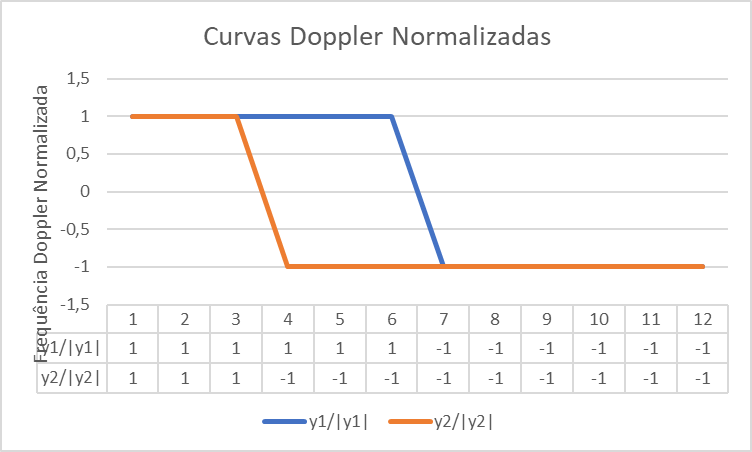
\includegraphics[width=0.8\linewidth]{figs/Metodologia/image007.png}
    \caption{Exemplo de curvas Doppler normalizado com dados gerados artificialmente}
    \label{fig:Doppler_norm_MET}
\end{figure}

Usando as transições das curvas normalizadas, procura-se por transições positivo$\rightarrow$negativo consecutivas, pois a mais recente provavelmente indica o sentido em que a pessoa caminha. Por exemplo, a figura \ref{fig:Doppler_norm_MET} possui a transição de $y_2$ em $x=4$ e a de $y_1$ em $x=7$, o que indicaria que a pessoa entrou no ambiente definido pela antena $y_1$.
 
 \subsubsection{Combinando a travessia por comparação de tempo de pico RSSI com o Efeito Doppler} \label{section:RSSI+doppler_met}
 
O último caso estudado combina a comparação dos tempos de picos de potência de sinal RSSI e a comparação das transições positivo$\rightarrow$negativo da frequência Doppler para confirmar com mais exatidão a existência de um cruzamento de fronteira. A figura \ref{fig:RSSI_Doppler_norm_MET} combina as figuras \ref{fig:rssicurvesmet1} e \ref{fig:Doppler_norm_MET} em uma.

   \begin{figure}[h]
    \centering
    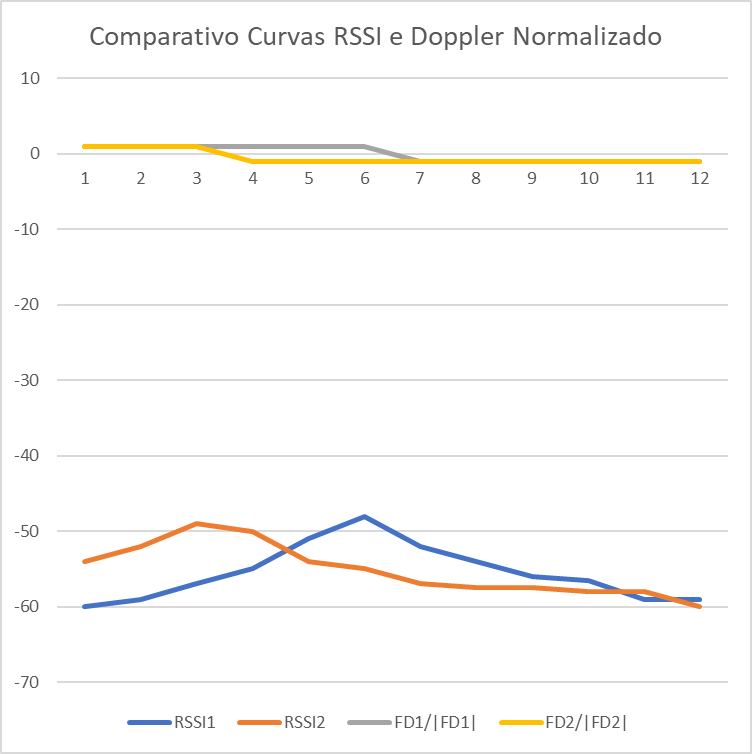
\includegraphics[width=0.8\linewidth]{figs/Metodologia/image009.png}
    \caption{Comparativo das curvas RSSI e Doppler Normalizado com dados gerados artificialmente}
    \label{fig:RSSI_Doppler_norm_MET}
\end{figure}

Na figura \ref{fig:RSSI_Doppler_norm_MET} observa-se que o pico $RSSI_1$ no instante $x=6$ ocorre ao mesmo tempo que a última leitura positiva de frequência Doppler $\frac{FD_1}{|FD_1|}$, e o pico $RSSI_2$ no instante $x=3$ ocorre ao mesmo tempo que a última leitura positiva de frequência Doppler $\frac{FD_2}{|FD_2|}$. Valores de pico de potência de sinal de resposta da TAG e transições de efeito Doppler acontecendo em momentos de tempo próximos indicam boa confiabilidade da sugestão de cruzamento de fronteira.

\begin{comment}
Desenvolvimento
\end{comment}

\chapter{Resultados\label{chap:Desenvolvimento}}

% Resumo opcional. Comentar se não usar.
\resumodocapitulo{resumo opcional}

texto

\subsection{Desenvolvimento}

texto \cite{vogt2002multiple}




\begin{comment}
Conclusões
\end{comment}

\chapter{Conclusões} \label{chap:Conclusao}

\label{CapConclusoes}

Os resultados obtidos foram promissores para os critérios de decisão de comparação de picos de potência de sinal RSSI e de comparação do último valor de RSSI. Ambos obtiveram eficiência observada de $100\%$. Estes resultados, apesar de muito bons, podem ser validados de forma melhor com uma amostra de testes maior do que 10 transições. Dessa forma, novos testes com mais dados podem ser conduzidos.

Os resultados obtidos com o critério de transição por comparação de frequência Doppler foram abaixo do esperado, dado o resultado surpreendente do teste preliminar da sessão \ref{sect:testepreliminar}. Esperava-se uma eficiência maior que $80\%$ de acerto, entretanto, este modelo obteve apenas $70\%$ de acerto. Como há evidência de que este método pode funcionar com boa taxa de acerto no teste preliminar, provavelmente este método pode ser corrigido para obter maior eficiência.

O resultado obtido com a união do critério de comparação de picos e de efeito Doppler teve rendimento abaixo do esperado, com apenas $70\%$ de eficiência, nivelando a eficiência dos dois métodos dos quais é composto pelo pior caso. Isso provavelmente se deve ao fato de que ele necessita que tanto o pico de RSSI quanto a transição de valores positivos para negativos do Efeito Doppler aconteçam ao mesmo tempo para registrar uma transição. Caso a leitora perca um dos eventos, este método não contabiliza a mudança de ambiente. Este método pode ser flexibilizado para aceitar ambos os critérios com lógica "OU" ao invés de lógica "E". Isso permitiria, talvez, uma taxa de acerto muito maior do que os outros métodos.

Os testes de mediana e média foram feitos sem muitas expectativas, e renderam resultados pouco expressivos - ambos obtiveram rendimento abaixo de 50\%. Estes dois métodos são muito lentos para a velocidade média com que uma pessoa atravessa uma porta. Eles possuem potencial, entretanto, como métodos de correção para os outros, em casos onde todo o ambiente possui cobertura de sinal pelas antenas, pois sua natureza lenta acumula leituras repetidas durante longos períodos de tempo, e podem ser utilizados para detectar uma pessoa parada no interior de uma sala.

Este trabalho possui grande potencial de implementação em sistemas reais de ERP,EPC, especialmente em ambientes diferenciados, tais como a área cirúrgico-laboratorial. Esse tipo de ambiente exige um controle fino da temperatura, integrando inteligência artificial para controle preditivo, para que os \textit{setpoints} de condições ambientais sejam sempre atingidos em tempo mínimo e com a menor variação possível. Além disso, exigem um severo sistema se segurança e controle de acesso, onde o uso das mãos é indesejado por se tratar de ambientes com risco biológico envolvido.

Considerando os fins acadêmicos e de desenvolvimento tecnológico, o trabalho desenvolvido já possui grande valor, pois possui potencial para aprimoramento e possui diversas aplicações possíveis diferentes. Dado o sucesso dos resultados obtidos com os métodos de comparação do último valor RSSI e dos tempos de picos de potência do sinal de retorno, sistemas de ar condicionado específicos podem ser controlados utilizando dados gerados por aplicações como o programa desenvolvido. Alguns exemplos de aplicações diferentes do setor hospitalar são áreas de grande movimentação de pessoas (como estações de metrô - onde todos já possuem um bilhete com etiqueta RFID passiva embutida), ou locais onde o controle acurado de temperatura é o critério mais importante, como um \textit{datacenter} ou laboratório de química.


\section{Perspectivas Futuras}

Este trabalho inovou nos métodos de identificação de mudança de ambiente em relação aos seus antecessores \cite{TG2013OliveiraERocha} \cite{TG2015RaissaERenata}. A nova abordagem na aplicação e nos algoritmos abre espaço para a aplicação de novas técnicas. Em especial destacam-se a lógica difusa, ou lógica \textit{fuzzy} \cite{yen1999fuzzy}, e a implementação de filtros preditivos, como o filtro de Kalman \cite{welch1995introduction}.

A lógica \textit{fuzzy} pode ser usada para aprimoramento do critério de decisão sobre em qual lado da porta ou passagem o portador da TAG se encontra. Já os filtros preditivos, seja o filtro de Kalman ou outro, podem ser úteis na hora de coletar os dados para obter leituras mais precisas e acuradas, tornando o processo de decisão mais confiável.

É aconselhado também buscar outras abordagens, como o LANDMARK \cite{bekkali2007rfid}, que tem o intuito de criar um mapa do ambiente em que se deseja monitorar as pessoas, e por meio dos padrões de magnitude dos sinais estima o local exato dentro de uma sala onde a pessoa se encontra.

Para finalizar, o desenvolvimento de uma integração com sistemas ERP,EPC é altamente recomendado, para que os estimadores de localização e contabilização da quantidade de pessoas presentes possam ser integrados em sistemas supervisórios comerciais, sistemas de controle de ar condicionado e sistemas de controle de acesso.

\begin{comment}
Bibliografia
\end{comment}


\renewcommand{\bibname}{REFERÊNCIAS BIBLIOGRÁFICAS}
\addcontentsline{toc}{chapter}{REFERÊNCIAS BIBLIOGRÁFICAS}

\bibliographystyle{abnt-num}
\bibliography{bibliography}


\begin{comment}
Anexos
\end{comment}


\anexos
\makeatletter
% não retirar estes comandos
\renewcommand{\@makechapterhead}[1]{%
  {\parindent \z@ \raggedleft \setfontarial\bfseries
\LARGE \thechapter. \space\space
\uppercase{#1}\par
\vskip 40\p@
}
}
\makeatother

\begin{comment}
Anexo I: Descrição do CD
\end{comment}



\chapter{Descrição do conteúdo do CD}

\label{AnCD}

Descrever CD.


\refstepcounter{noAnexo}

\begin{comment}
Anexo II: Programas Utilizados
\end{comment}



\chapter{Programas utilizados}

O programa desenvolvido em linguagem de programação C\# foi apresentado neste Anexo. Os arquivos de cada classe do formato ".CS" foram organizados em ordem alfabética, seguindo o padrão:

\begin{itemize}
    \item Ambient.cs
    \item Antenna.cs
    \item Cardholder.cs
    \item Curve.cs
    \item FileHandler.cs
    \item Program.cs (Main)
    \item Project.cs
    \item Transition.cs
\end{itemize}


\refstepcounter{noAnexo}

\begin{comment}
Acrescente mais anexos conforme julgar necessário.
\end{comment}

\end{document}
